\subsection{KENN with different encoders: DistilBERT vs BERT} \label{distilbert_vs_bert}
Choosing the right language model is always important to determine the performance of the final model, especially if the goal is to compete with state-of-the-art solutions. This experiment aims to compare the behavior of KENN when dealing with networks based on encoders with different capabilities, which in our case are DistilBERT and BERT.

\subsubsection{Setup}
The models used for this experiment are trained using the \textit{Setup B}. The experimental parameters chosen are the following:
\begin{itemize}
    \item \textbf{KB modes:} Bottom Up, Top Down and Hybrid
    \item \textbf{initial clause weight:} 2.0
    \item \textbf{fixed clause weights}
    \item \textbf{encoder:} DistilBERT and BERT, with adapters
    \item \textbf{loss function:} Binary Cross-Entropy, with the weights of positive examples set to 1
\end{itemize}
This results in a total of 6 configurations. The choice of using fixed clause weights set to 2.0 comes from the previous experiments since it has been observed that higher weights led to higher boosts in the early stage of the training. The experiments are evaluated in terms of \textit{macro f1 examples} by averaging the performance obtained from 3 random seeds per model.

\subsubsection{Results on FIGER}
We can start by comparing the performance obtained by the baseline model with different encoders. Looking at the graph in Figure~\ref{fig:wandb_figer_baseline_distilbert_vs_bert}, we can observe a significant gap between the models. The difference, which is larger at the beginning, persists for the duration of the training and shows the major capabilities of BERT. The final models reach a score of 0.9155 and 0.8911 for BERT and DistilBERT, respectively.
\begin{figure}[bth]
    \centering
    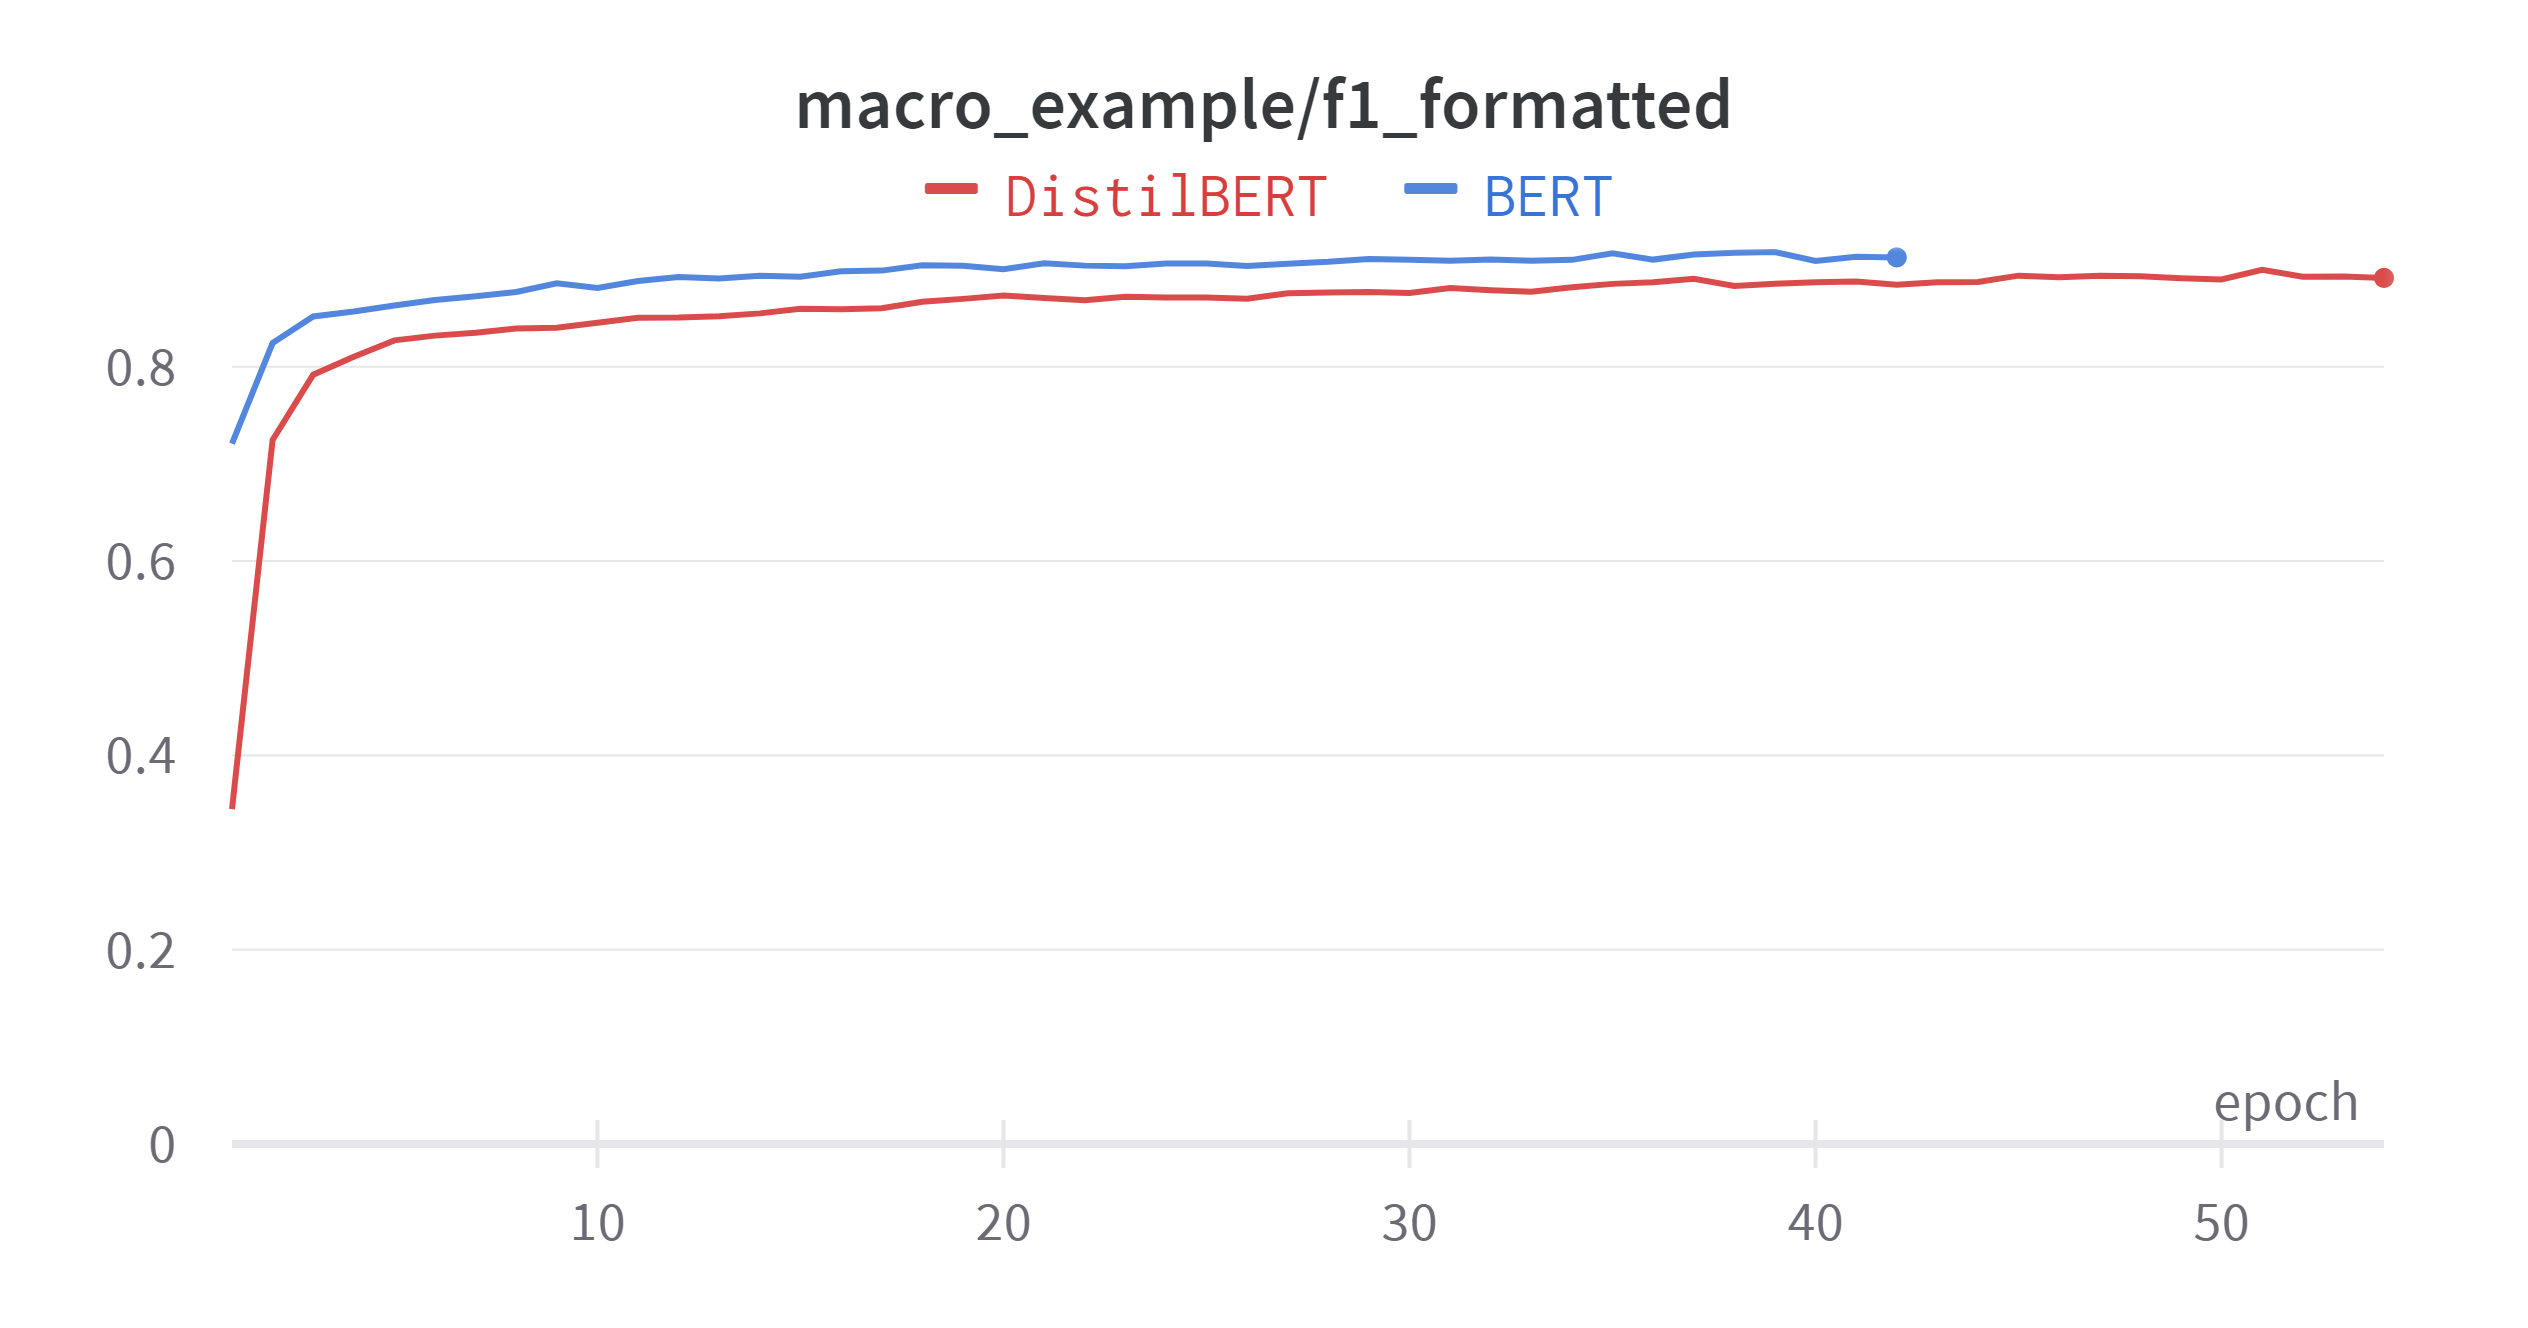
\includegraphics[width=.8\linewidth]{figures/wandb_figer_baseline_distilbert_vs_bert.png}
    \caption{Baseline DistilBERT vs Baseline BERT in terms of \textit{macro f1 examples} on the dev set of FIGER}
    \label{fig:wandb_figer_baseline_distilbert_vs_bert}
\end{figure}

Now that the superiority of BERT has been confirmed, we can proceed with the comparison between the baseline and KENN-based models. In Figures~\ref{fig:wandb_figer_kenn_distilbert} and \ref{fig:wandb_figer_kenn_bert} are presented the performance obtained with DistilBERT and BERT, respectively. As we can see, the behavior of KENN is completely different depending on the encoder. Starting from DistilBERT, the initial boost given by KENN is clearly visible, especially when comparing the baseline to the Hybrid model. However, as already discussed in the quantitative analysis, this boost vanishes in the rest of the training when the models converge. When using BERT, instead, the baseline model is the one that has the best start. While Top Down has a similar training trend even at the beginning, Bottom Up and Hybrid are always inferior.

\begin{figure}[bth]
    \centering
    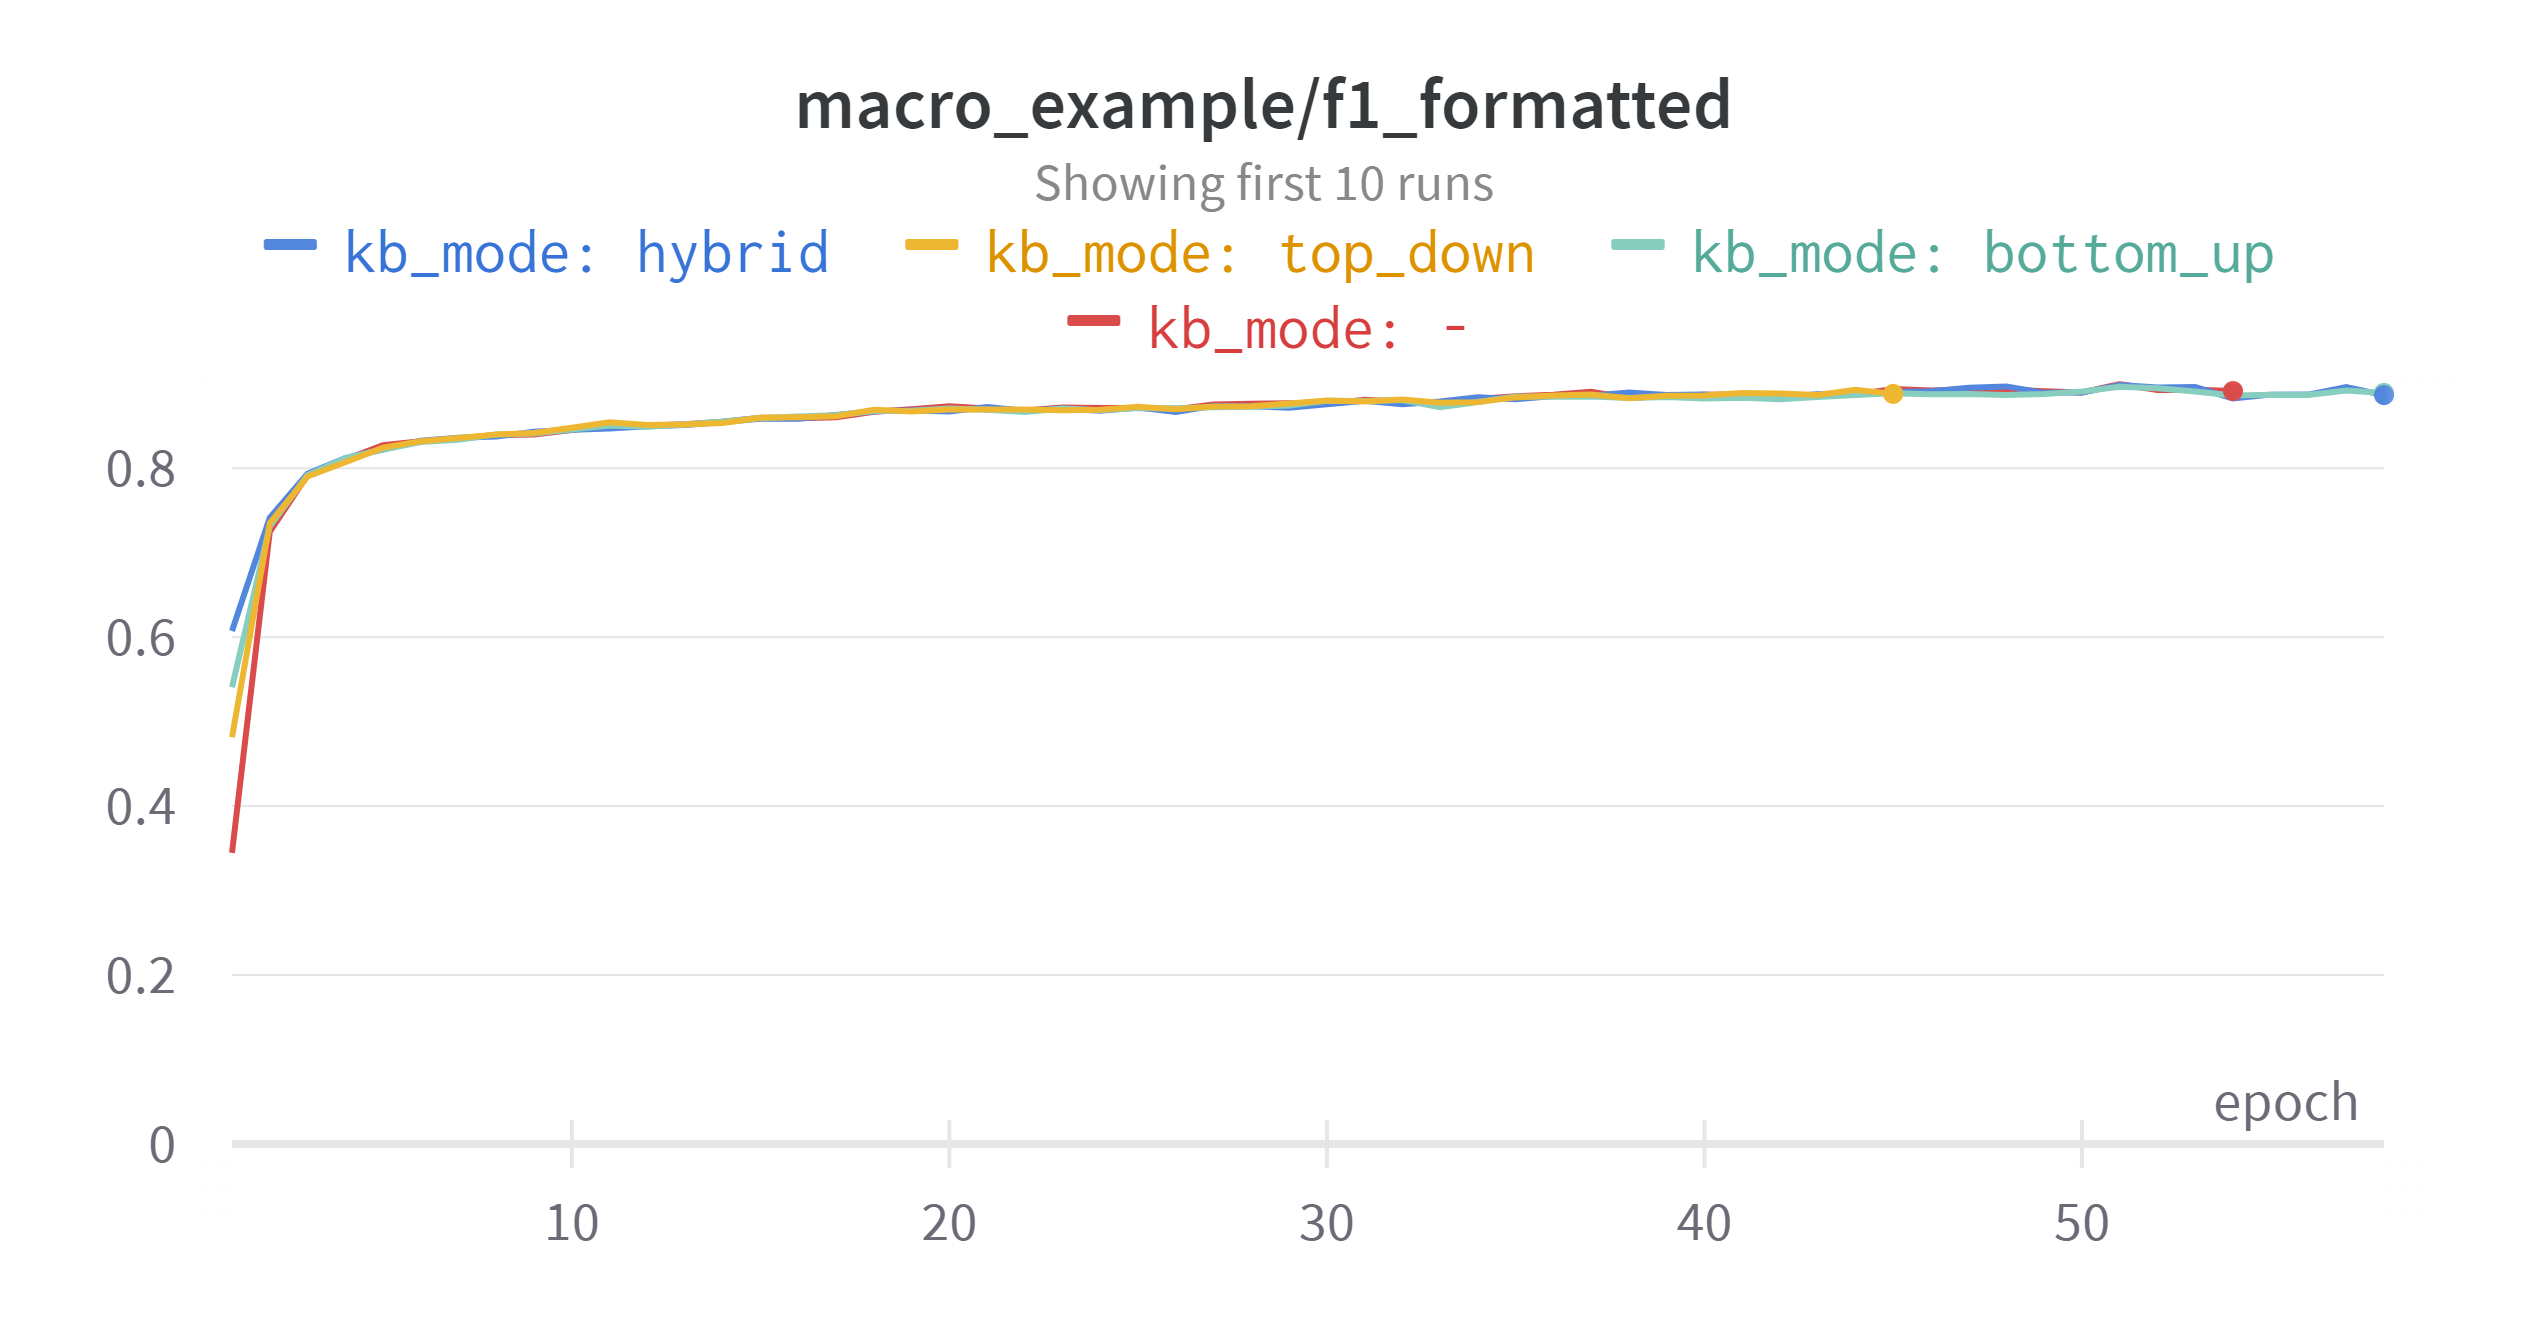
\includegraphics[width=.8\linewidth]{figures/wandb_figer_kenn_distilbert.png}
    \caption{Baseline DistilBERT vs KENN DistilBERT in terms of \textit{macro f1 examples} on the dev set of FIGER.}
    \label{fig:wandb_figer_kenn_distilbert}
\end{figure}

\begin{figure}[bth]
    \centering
    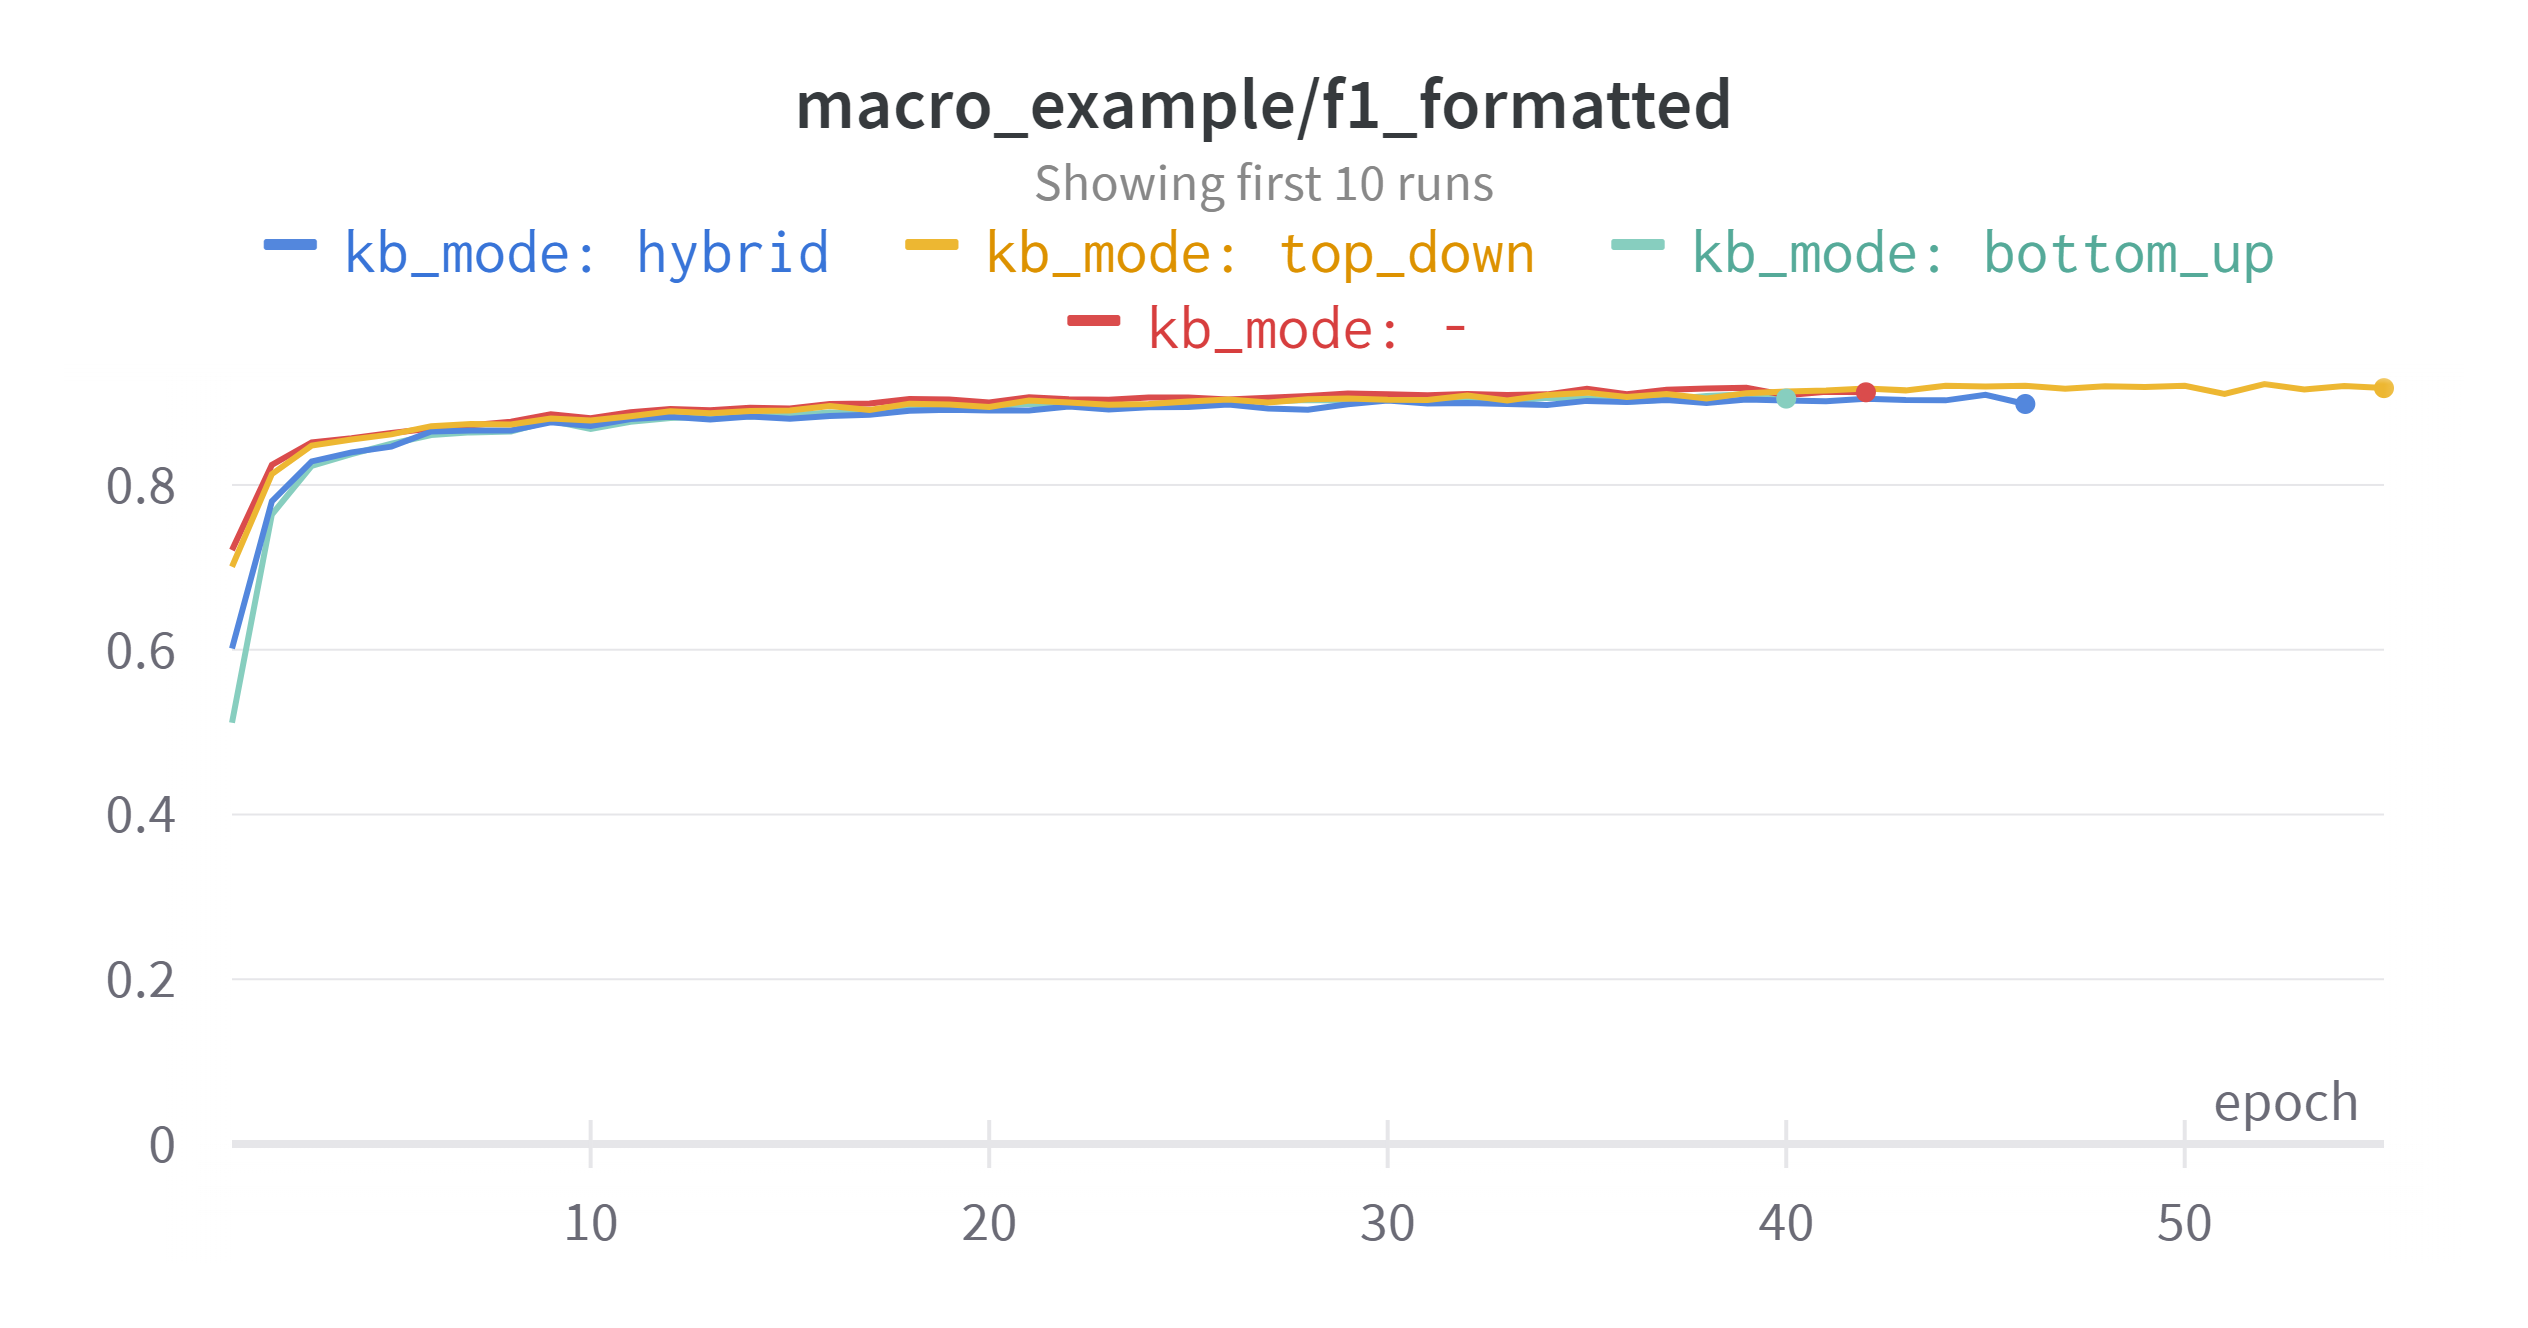
\includegraphics[width=.8\linewidth]{figures/wandb_figer_kenn_bert.png}
    \caption{Baseline BERT vs KENN BERT in terms of \textit{macro f1 examples} on the dev set of FIGER.}
    \label{fig:wandb_figer_kenn_bert}
\end{figure}




\subsubsection{Results on BBN}
Figure~\ref{fig:wandb_bbn_baseline_distilbert_vs_bert} compares DistilBERT and BERT when using the baseline model. Even this dataset confirmed the superiority of BERT, which reached the score of 0.9047, while DistilBERT's score is 0.8845.

\begin{figure}[bth]
    \centering
    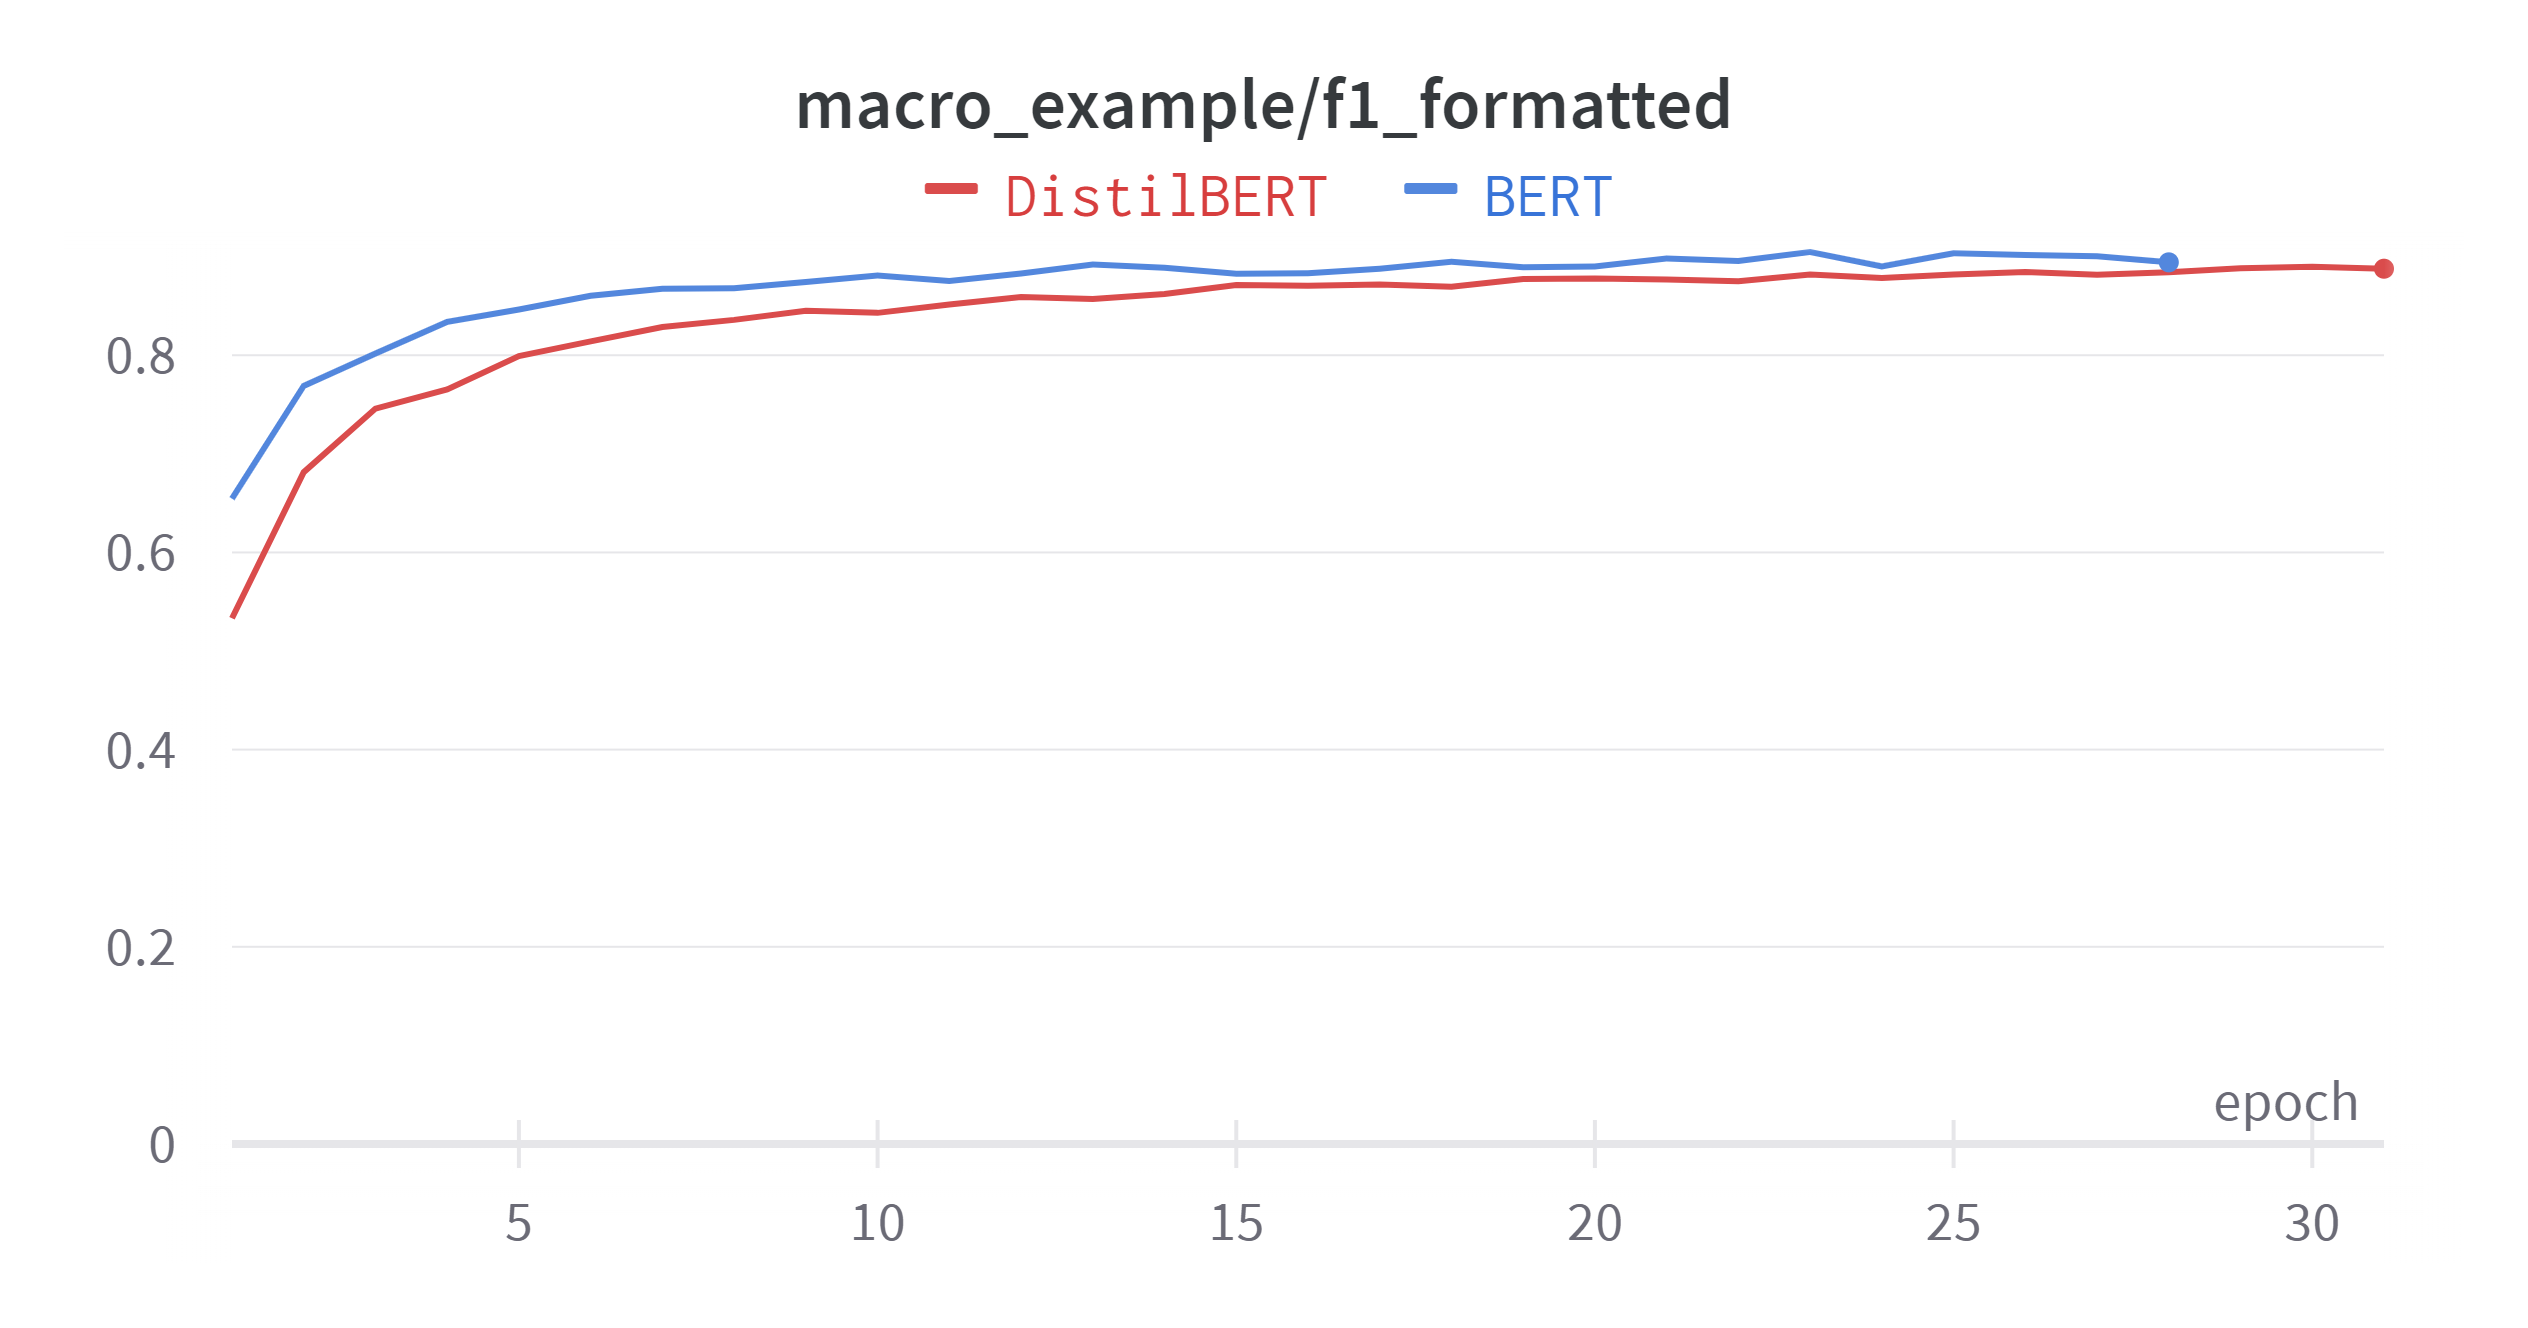
\includegraphics[width=.8\linewidth]{figures/wandb_bbn_baseline_distilbert_vs_bert.png}
    \caption{Baseline DistilBERT vs Baseline BERT in terms of \textit{macro f1 examples} on the dev set of BBN.}
    \label{fig:wandb_bbn_baseline_distilbert_vs_bert}
\end{figure}

The trends of KENN-based models compared to the baseline when using DistilBERT and BERT are available in Figures~\ref{fig:wandb_bbn_kenn_distilbert} and \ref{fig:wandb_bbn_kenn_bert}, respectively. Looking at the graphs, we can make the same observation done for FIGER: the logical knowledge gives an initial boost only when using DistilBERT. Moving on to BERT, except Bottom Up, which has a slower start, the other models have very similar training trends.

\begin{figure}[bth]
    \centering
    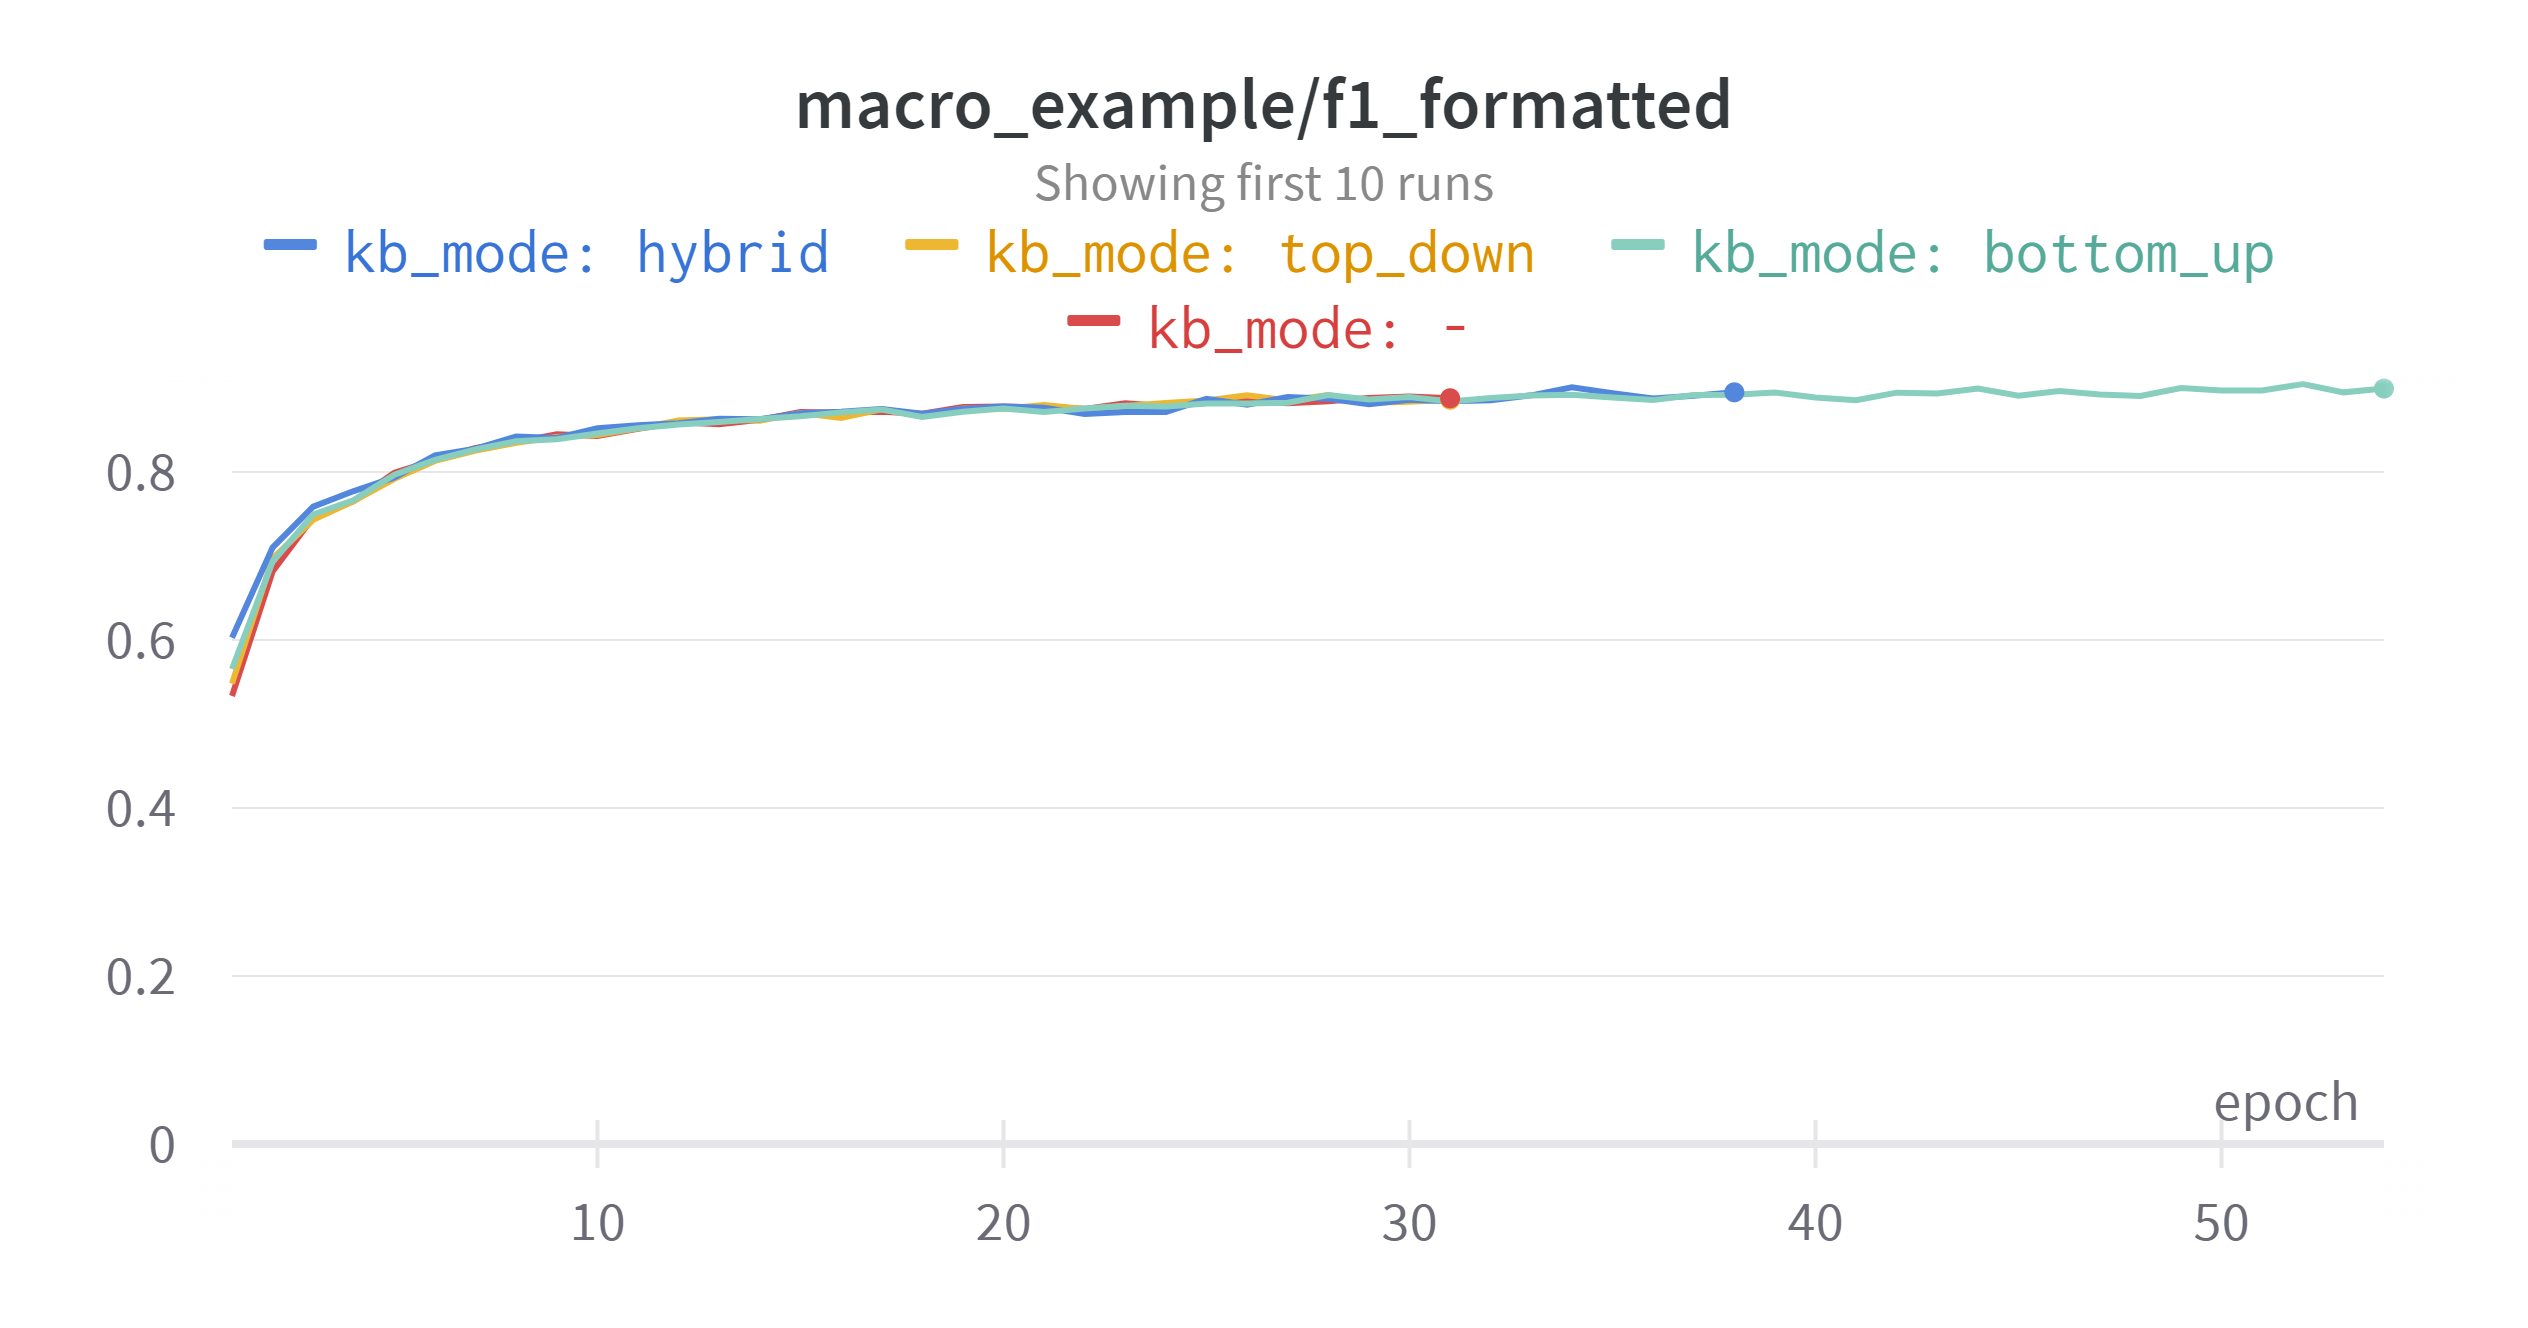
\includegraphics[width=.8\linewidth]{figures/wandb_bbn_kenn_distilbert.png}
    \caption{Baseline DistilBERT vs KENN DistilBERT in terms of \textit{macro f1 examples} on the dev set of BBN.}
    \label{fig:wandb_bbn_kenn_distilbert}
\end{figure}

\begin{figure}[bth]
    \centering
    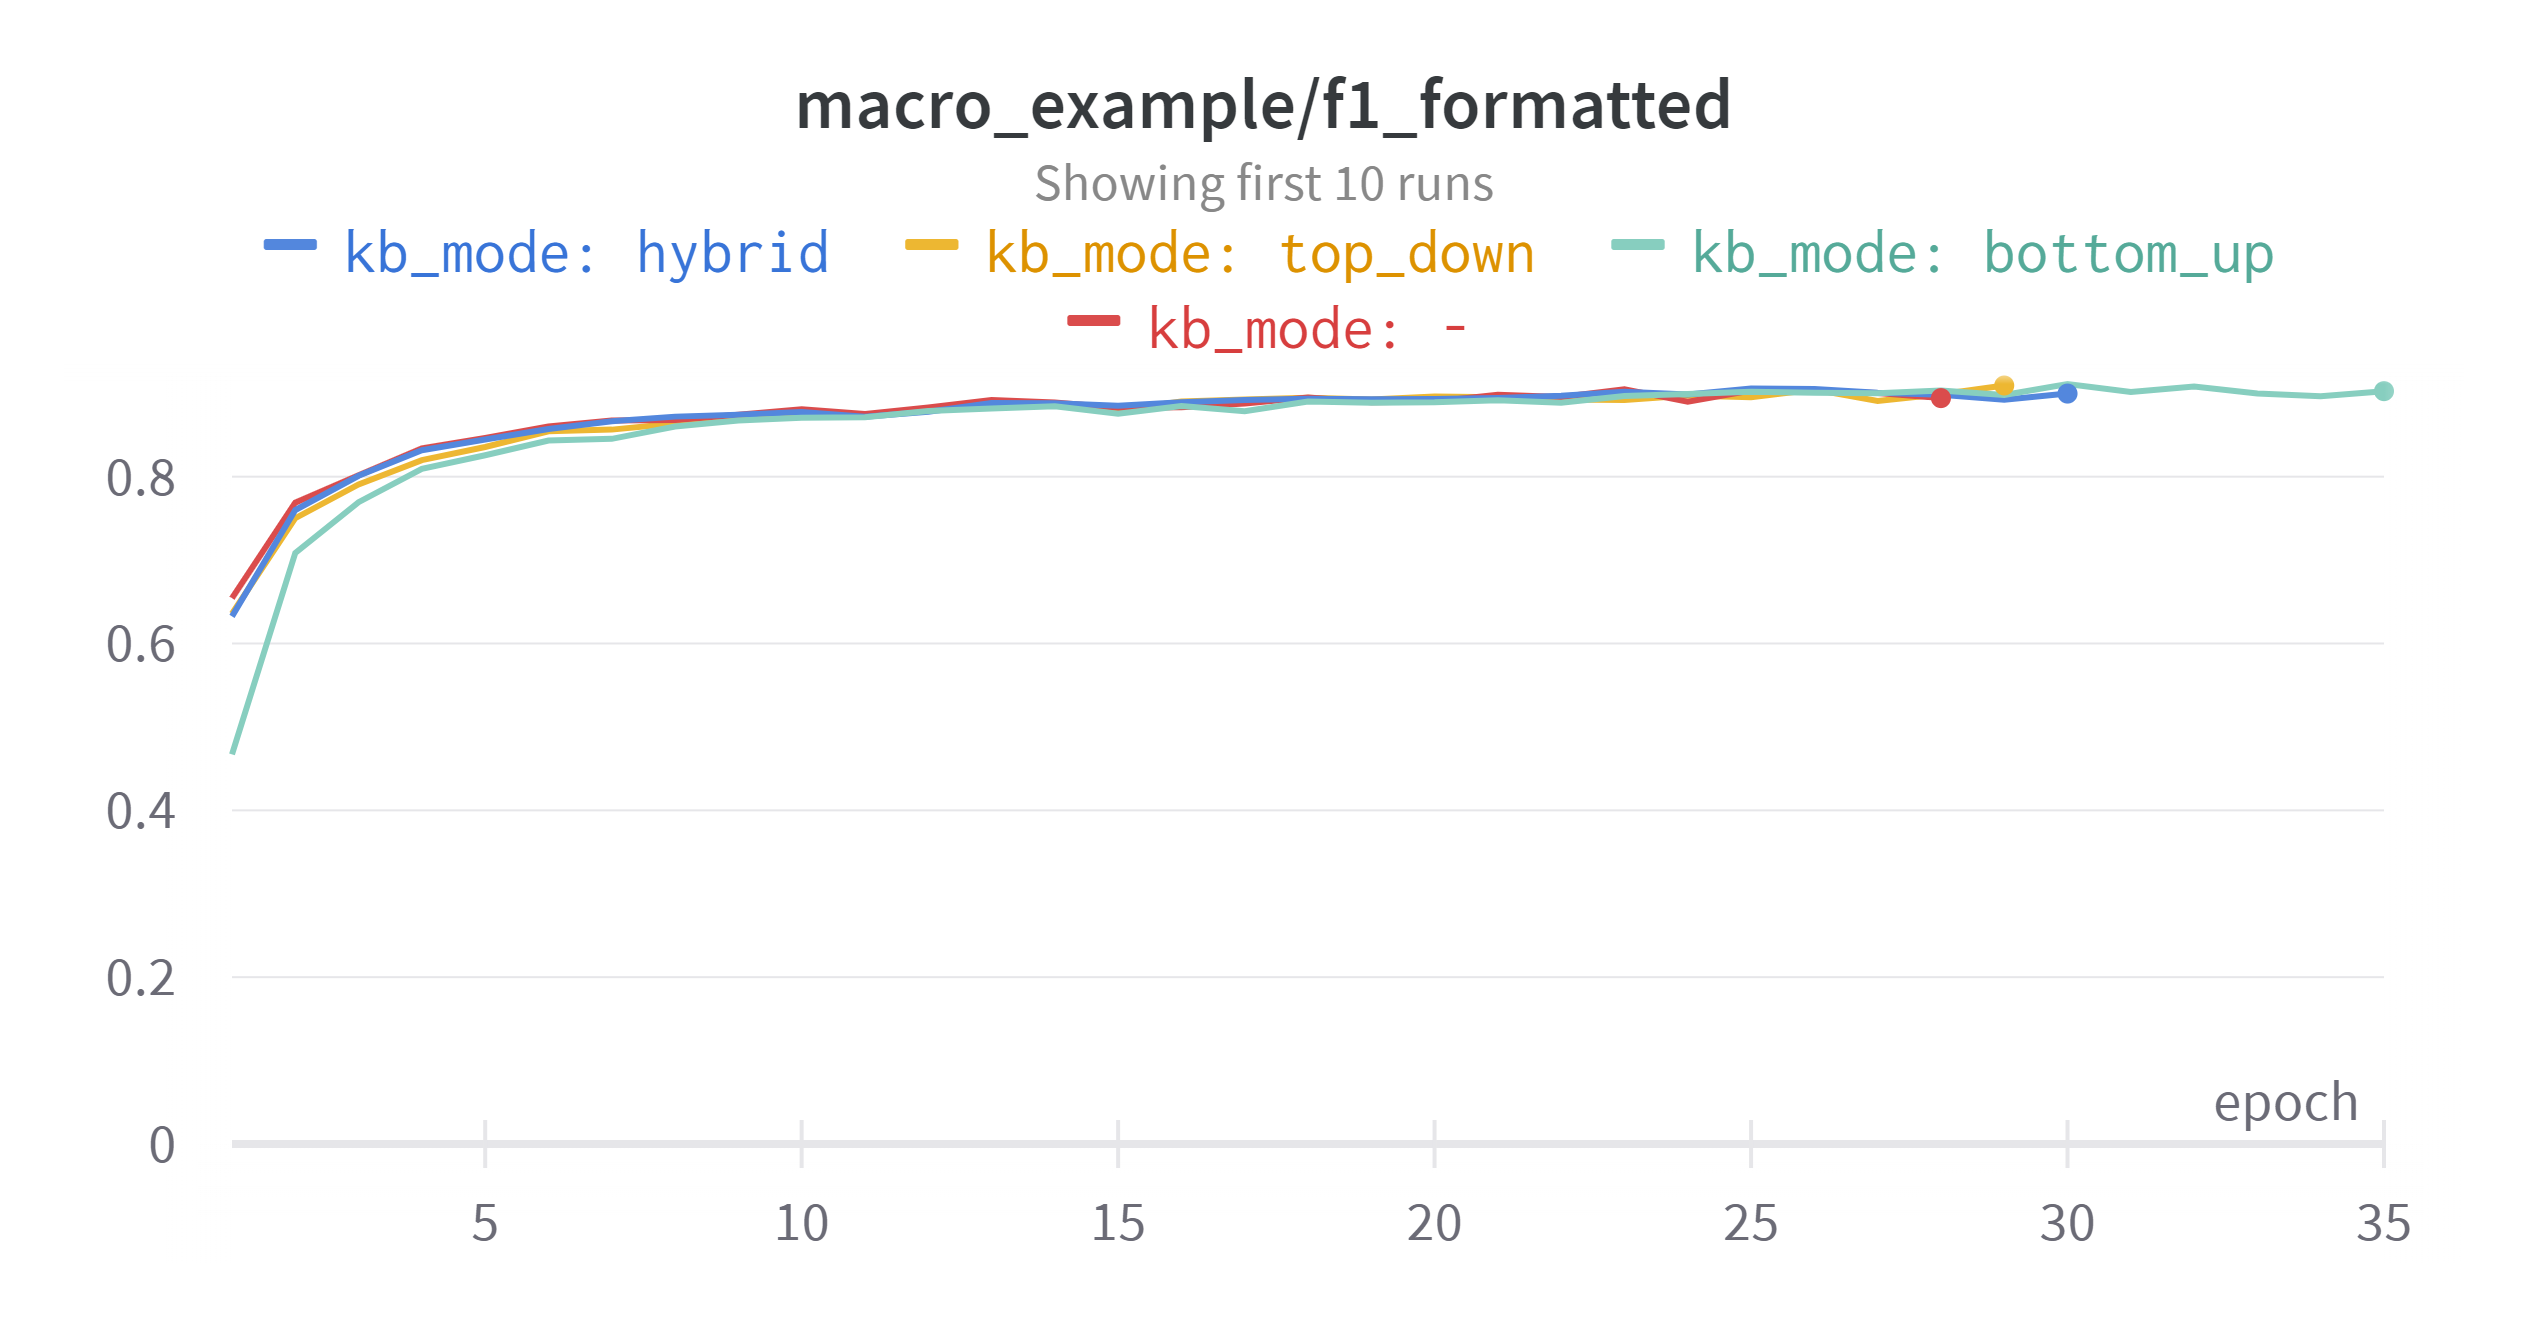
\includegraphics[width=.8\linewidth]{figures/wandb_bbn_kenn_bert.png}
    \caption{Baseline BERT vs KENN BERT in terms of \textit{macro f1 examples} on the dev set of BBN.}
    \label{fig:wandb_bbn_kenn_bert}
\end{figure}

\subsubsection{Conclusion}
The results obtained on the two datasets highlighted that the benefits of the logical knowledge are visible only in the early stage of the DistilBERT-based models. The fact that KENN worsened the performance of the BERT-based models was quite unexpected. Except for the Top Down mode, it seems that the injection of logical knowledge disturbed the learning process of the other models, especially at the beginning of the training. An explanation for this behavior can be found in the words of KENN's authors, which said that KENN has more difficulties when integrated into neural networks that are already capable to satisfy the provided clauses, since any bias is introduced towards their satisfaction~\cite{daniele2021neural}.

In our case, we observed that the performance of the baseline model was substantially improved when using BERT. For this reason, it may be possible that BERT, which provides a richer text representation than DistilBERT, is already able to implicitly learn from data the hierarchical information without the need for logical knowledge. Furthermore, we can think about the differences between the KB modes to explain why Top Down has higher performance than Bottom Up: while the knowledge provided by a Bottom Up clause could be learned from data (i.e., the model learns that a subtype always co-occur with its supertype), Top Down clauses could introduce more bias into the learning process, thus adding new solutions to the Hypothesis Space as said in~\cite{daniele2021neural}.